%%==================================================
%% chapter02.tex for BIT Master Thesis
%% modified by yang yating
%% version: 0.1
%% last update: Dec 25th, 2016
%%==================================================
\chapter{基于多重校验的时间隐通道构建方法研究}
\label{chap:hash}

对于VoLTE中基于主动丢包的时间隐通道来说,丢包噪声干扰了隐通道鲁棒性。但受限于抗检测性指标的约束,时间隐通道主动丢包比例较低,因此需要更有效的鲁棒性策略降低噪声干扰。本章主要介绍通过多重校验的方式,构建低误码率高鲁棒性的时间隐通道。

%在下方加入各小节内容
\section{概述}
\label{chap:hash:overview}

通过主动丢包的方式构建时间隐通道,为保证传输隐蔽性,主动丢包率较低。通过分析抓包数据,VoLTE视频信道丢包率高于LTE网络的QCI目标值,时间隐通道的信噪比较低。VoLTE中的丢包类型,分为长度为1的随机丢包噪声,以及连续丢包噪声。对于密度较低的随机丢包噪声,通过嵌入校验信息即可有效区分噪声及信号;而对于连续丢包噪声,单组校验信息已经无法有效鉴别,需要通过多组校验信息中的冗余数据进行鉴别。

基于多重校验的时间隐通道构建方法,主要研究在码字、符号及映射矩阵三个层次中,分别添加校验过程,逐层降低噪声强度。在该时间隐通道构建方法中,采用了码字间校验、码字自校验以及符号间校验三个校验层次。结合HASH摘要算法、CRC散列算法及异或校验算法几种方式,在Excellent场景中实现了极低误码率,有效降低了Good场景中的平均误码率。

该方法的创新点如下:
\begin{itemize}
	\item 提出了基于多重校验的时间隐通道构建方法,有效降低了误码率水平;
	\item 设计了包含码字间校验、码字自校验及符号间校验三个层次的校验方式,逐层降低噪声水平;
	\item 支持传输参数调整,在增强鲁棒性的同时保证传输性能。
\end{itemize}

通过实验测试证明,通过调整该时间隐通道的各项传输参数,能够在传输性能、误码率水平及抗检测能力方面实现平衡,在可用性及有效性方面实现了提升。
\section{研究背景和动机}
\label{chap:hash:motivation}

本节对该方法中涉及的相关背景进行介绍,包括网络噪声对时间隐通道的干扰方式,以及基于码字间校验的鲁棒性策略。其中,网络噪声对时间隐通道的干扰,主要分析了不同类型的网络噪声对码字鉴别的干扰情况,并提出了问题的解决方法。基于码字间检验的鲁棒性策略,提出了建立码字间的校验关系,提高校验信息利用率的方法。

\subsection{网络噪声对时间隐通道的干扰}
\label{chap:hash:motivation:noise}

由图\nref{fig:2:pmf-dropout}可知,VoLTE视频通话中丢包长度为1的突发丢包占比在50\%左右,而其余的均为连续丢包事件。通过CRC检错码等方式,对离散的随机丢包噪声具有较好的抑制作用,而在连续丢包噪声干扰中,数据码字及校验码字出现误匹配概率较高,导致码字鉴别准确率较低,最终传输结果的误码率升高。

\insertFigure{
	\begin{figure}
		\centering
        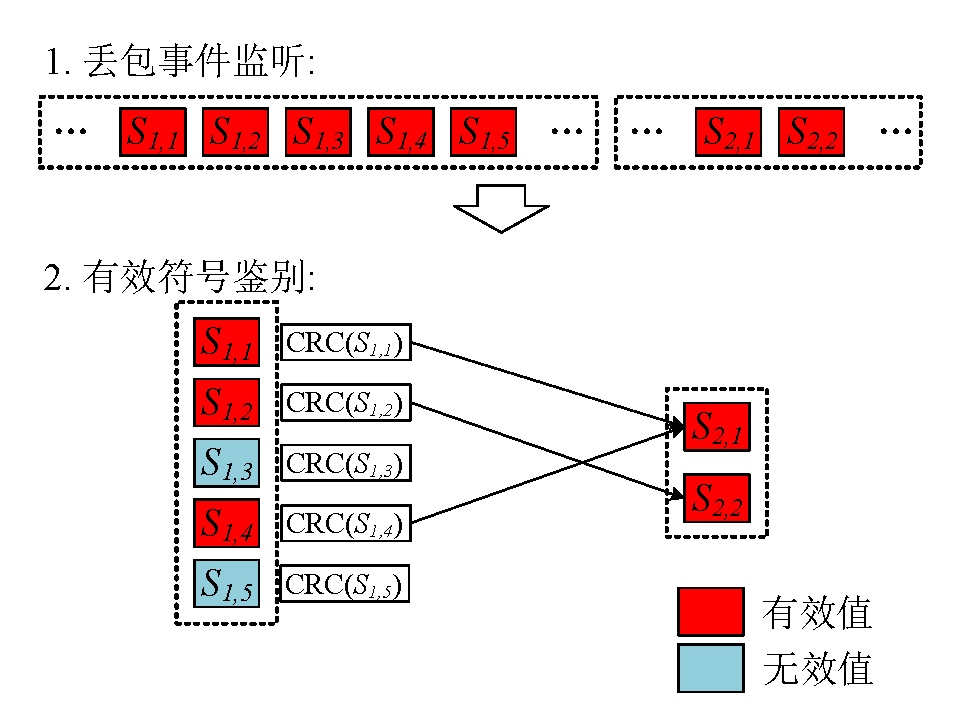
\includegraphics[width=0.7\textwidth]{chapters/chapter5/figures/crc-continuous.pdf}
        \caption{连续丢包对鉴别过程的影响示意图}
        \label{fig:5:crc-continuous}
	\end{figure}
}

如图\nref{fig:5:crc-continuous},存在连读丢包的情况下,通过CRC进行有效符号鉴别,存在明显的校验能力退化。第一组$S_{1}$为待验证的数据符号,第二组$S_{2}$为可能的校验符号,在第一步的丢包事件监听中,无法区分符号的有效性,因此所有的符号作为候选值进入第二步。在有效符号鉴别过程中,依次计算CRC($S_{1,i}$),并将结果与$S_{2,j}$比较,由于校验符号只是CRC散列结果的一部分,存在碰撞的概率较高。最终的鉴别结果,只能识别出部分网络噪声。由于缺乏额外的鉴别信息,无法进一步判别噪声,导致解调结果出现误码。

理想情况下,按照\nref{chap:zigzag:model:modulation:crc}中设计的鲁棒性方案,当数据组出现噪声而校验组无噪声时,产生误码的概率为$1/L_{Codeword}$,具备有效的鉴别能力。而实际场景中,校验组也会受噪声干扰,产生图\nref{fig:5:crc-continuous}中鉴别失效的结果。

\insertFigure{
	\begin{figure}
		\centering
        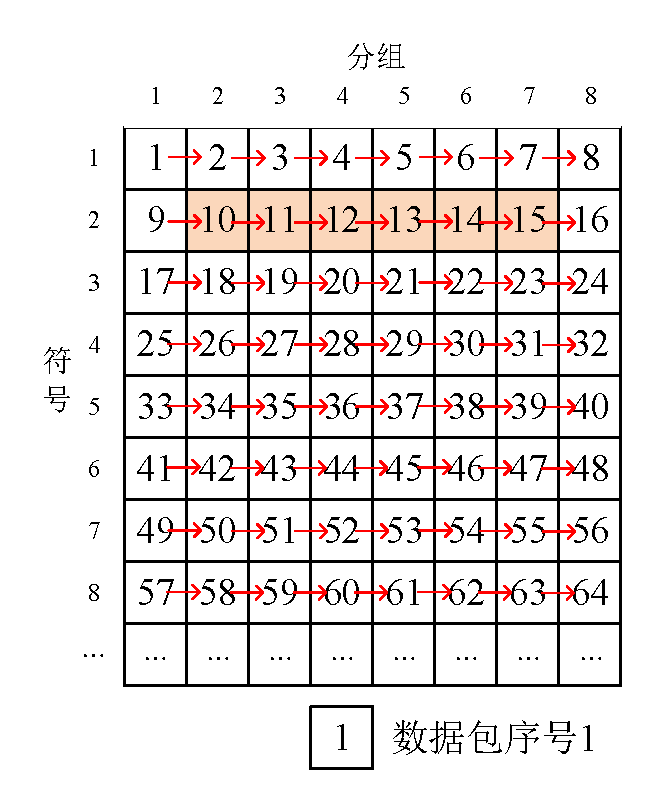
\includegraphics[width=0.45\textwidth]{chapters/chapter5/figures/row-matrix.pdf}
        \caption{符号-数据包序号映射矩阵示意图}
        \label{fig:5:row-matrix}
	\end{figure}
}

在VoLTE视频通话中,丢包时刻存在随机性,出现密集连续丢包的概率较低。因此,将连续丢包导出的符号分散,利用每组的校验能力,降低噪声干扰,是应对该类型噪声的可行办法。如图\nref{fig:5:row-matrix},矩阵中的位置为数据包序号,矩阵元素的列号为组号,行号对应符号。当出现连续丢包,如$10\sim 15$,经过该映射矩阵的处理,被分配到分组$2\sim 7$,有利于充分利用校验字段的校验能力,提高校验资源利用率。

\subsection{基于码字间校验的鲁棒性策略}
\label{chap:hash:motivation:robustness}

时间隐通道的鲁棒性策略中,包含喷泉码等无速率编码,结合多个码字之间的数据冗余,还原真实的消息内容,扩大了校验信息的作用范围。\nupcite{6296078}在区块链技术中,每一个区块中均含有前一个区块的HASH值,因此当链长达到一定规模时,起始区块的正确性越高。\nupcite{7467408}在基于主动丢包的时间隐通道中,由于噪声分布不均匀,添加码字间校验关系,利用低噪声的信息校验高噪声的数据,进一步提高校验信息利用率。

\insertFigure{
	\begin{figure}
		\centering
        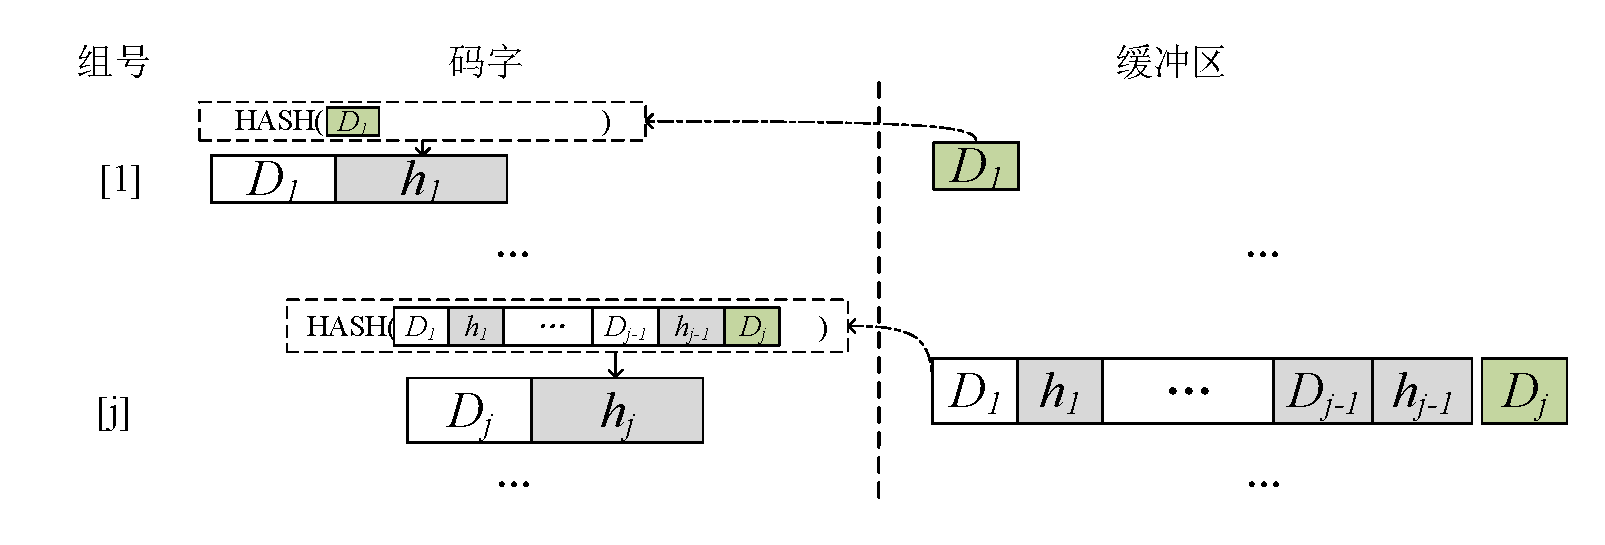
\includegraphics[width=0.95\textwidth]{chapters/chapter5/figures/chain-example.pdf}
        \caption{码字间校验结构示意图}
        \label{fig:5:chain-example}
	\end{figure}
}

如图\nref{fig:5:chain-example},码字间校验块$h_{j}$记录了数据缓冲区的校验结果。借助HASH函数的随机性和确定性,随着接收组数的增长,通过后接收码字中的码字间校验信息,验证已经接收到码字的正确性。即使部分的码字受噪声干扰,借助其它组中的低噪声有效信息,完成码字鉴别,降低噪声干扰强度。

码字间校验的HASH摘要,在计算时进行了加盐处理,通过结合用户自定义信息及RTP随机字段,提高了时间隐通道保密性。监听者监听到丢包事件后,无法正确恢复码字间校验块$h_{j}$,从而无法验证码字间校验关系,存在噪声干扰时无法区分噪声及信号,隐蔽消息得到保护。

\subsection{研究动机}
\label{chap:hash:motivation:motivation}

本时间隐通道构建方法,基本的调制方式为主动丢包,将调制产生的丢包隐匿在网络噪声中,通过多重校验的方式在解调过程中有效去噪,提高鲁棒性降低误码率。在多重校验的基础上,引入加盐及随机化过程,增加调制过程的随机度,增强隐蔽消息的保密性。

\insertFigure{
	\begin{figure}
		\centering
        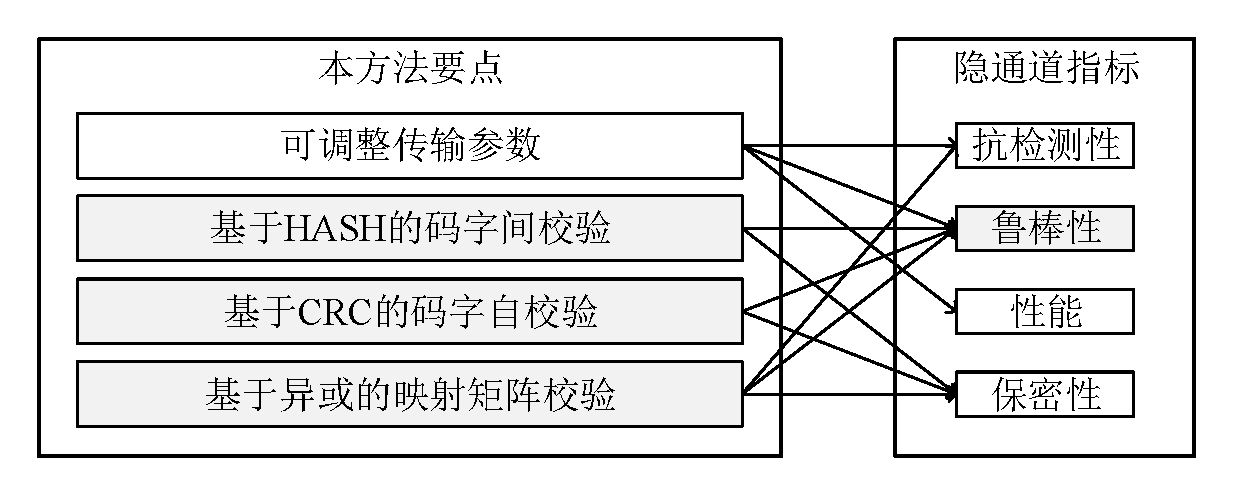
\includegraphics[width=0.8\textwidth]{chapters/chapter5/figures/chapter-struct.pdf}
        \caption{基于多重校验的时间隐通道构建方法研究要点与指标}
        \label{fig:5:chapter-struct}
	\end{figure}
}

如图\nref{fig:5:chapter-struct},本方法的要点主要有可调整传输参数、基于HASH的码字间校验、基于CRC的码字自校验及基于异或的映射矩阵校验。其中,可调整传输参数主要解决抗检测性、鲁棒性及传输性能之间的均衡问题。该方法中需要牺牲性能保证鲁棒性,因此通过调整传输参数实现各方面的统筹。基于HASH的码字间校验、基于CRC的码字自校验,主要提升时间隐通道的鲁棒性,同时提高隐蔽消息的保密性。基于异或的映射矩阵校验,通过构建具有校验能力的映射矩阵,在分散丢包位置的基础上提高鲁棒性。
\section{基于多重校验的时间隐通道构建方法}
\label{chap:hash:results}

本节对该时间隐通道构建方法进行总体介绍,首先在整体的设计架构方面进行介绍,然后对调制流程及数据转换过程进行介绍,最后对解调过程及数据转换进行介绍。

\subsection{设计架构}
\label{chap:hash:results:model}

\insertFigure{
	\begin{figure}
		\centering
        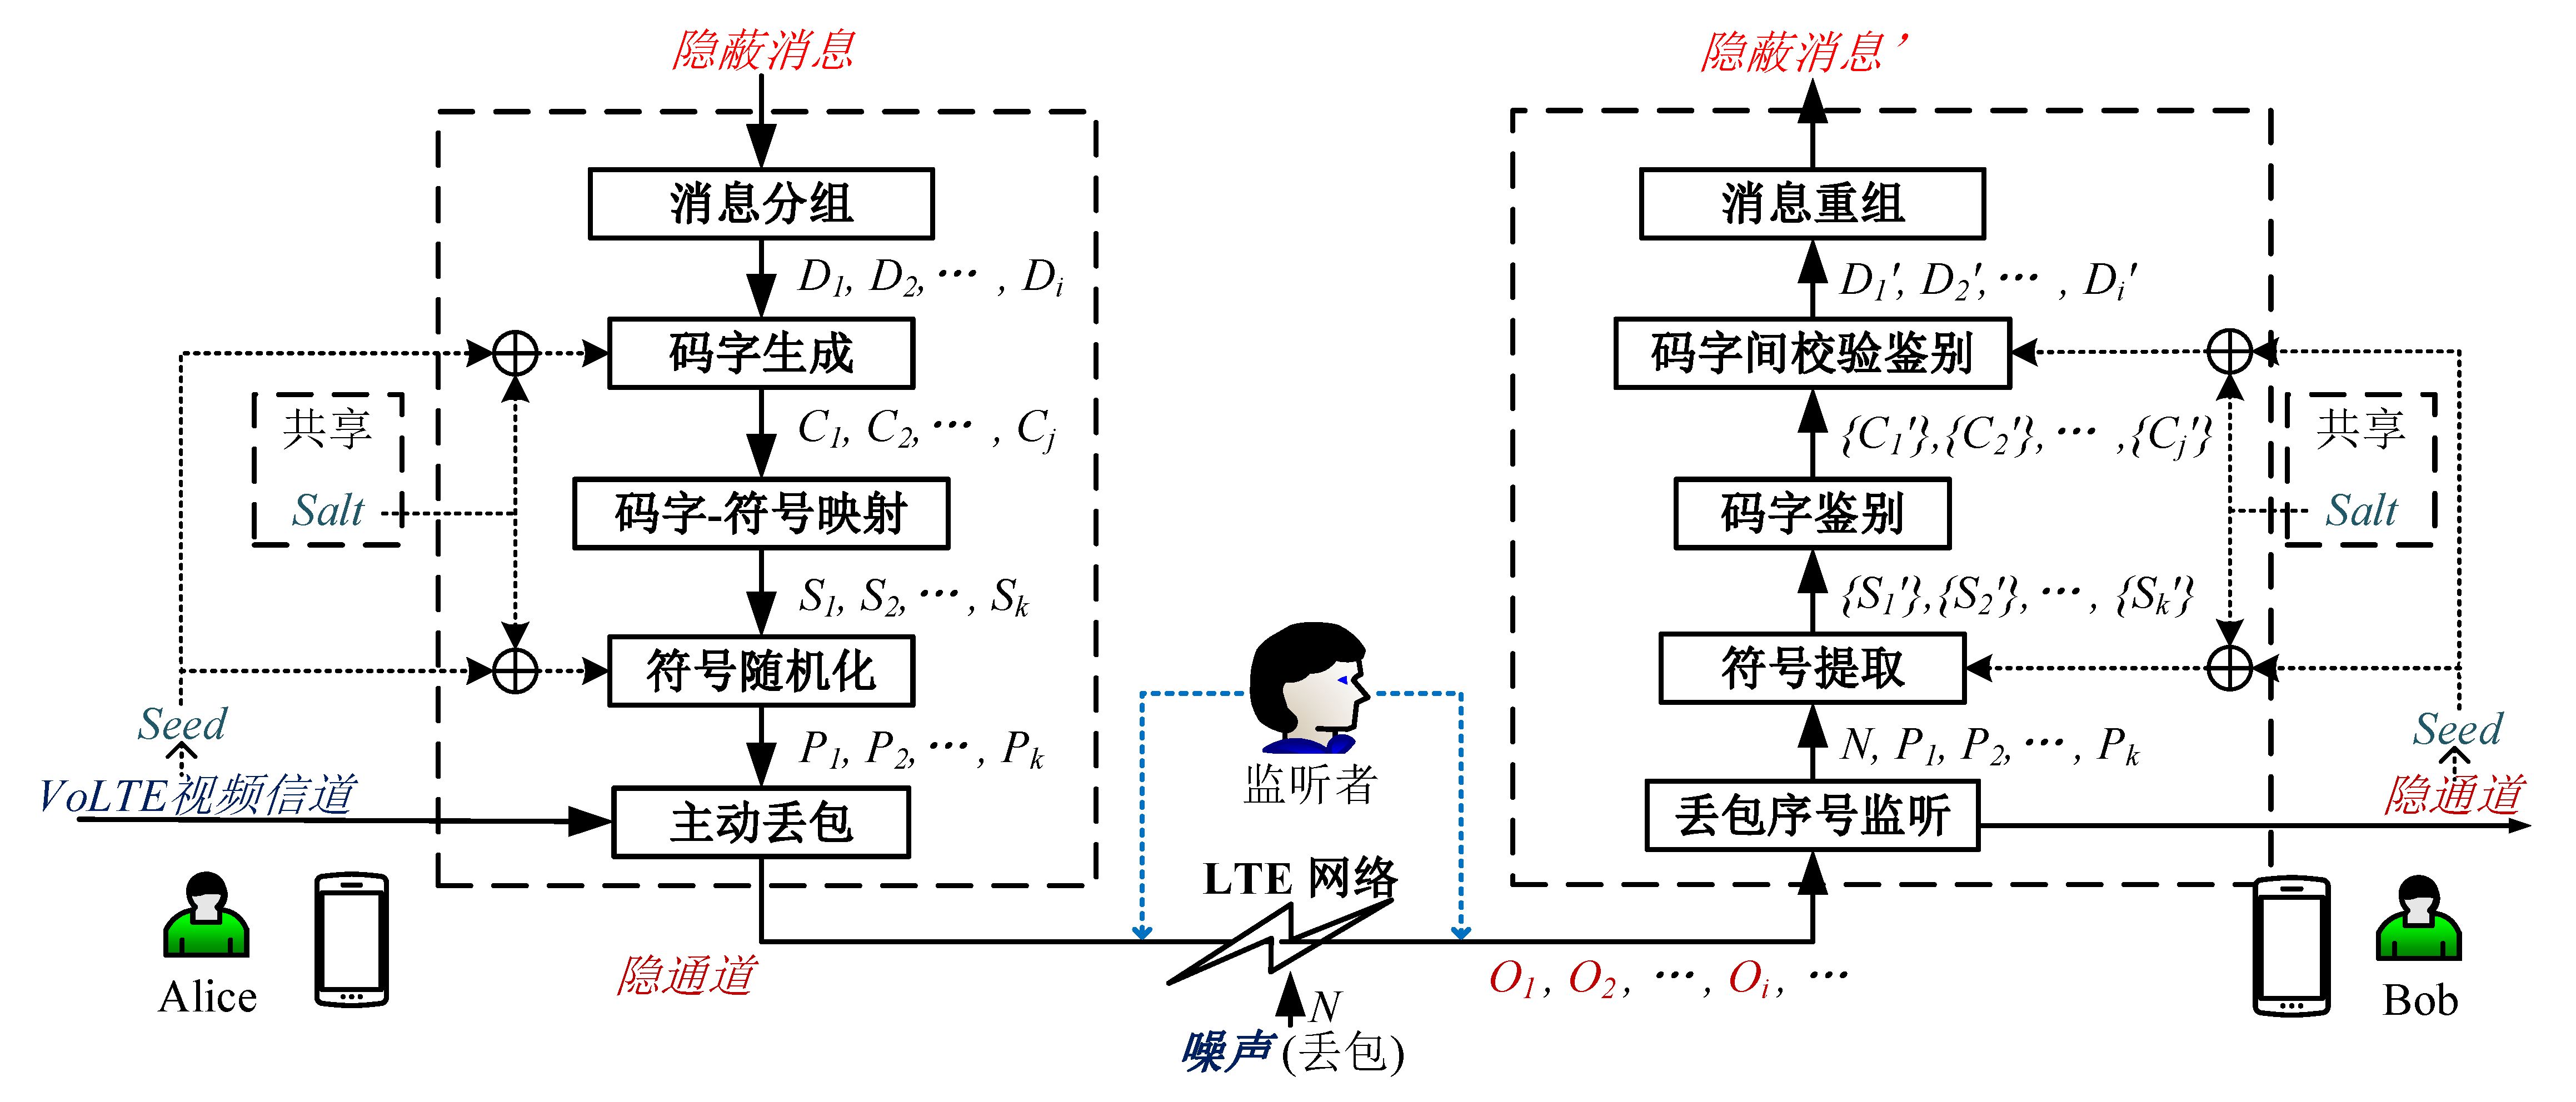
\includegraphics[width=0.99\textwidth]{chapters/chapter5/figures/system-model.pdf}
        \caption{基于多重校验的时间隐通道设计架构图}
        \label{fig:5:system-model}
    \end{figure}
}

该时间隐通道构建方法的设计架构如图\nref{fig:5:system-model},对于发送方Bob和接收方Alice来说,需要通过该时间隐通道发送隐蔽消息。为保证较保密性,双方约定一个共享的私有变量$Salt$,用于增加传输过程的随机性。发送方首先将隐蔽消息按照传输参数,进行消息分组,得到消息块$D_{i}$。接下来,码字生成过程借助私有$Salt$及RTP中的随机字段$Seed$,计算码字间校验信息及码字自校验信息,形成码字$C_{j}$。借助映射矩阵,将码字映射为符号$S_{k}$,也就是相对丢包位置。符号随机化过程对每一组的符号添加随机偏移量,并转换为要丢弃的数据包序号$P_{k}$。

宿主信道即VoLTE的视频信道,主动丢包过程将特定序号的数据包丢弃后,转变为时间隐通道,经过LTE网络传输后,到达接收方。监听者对LTE网络中的所有数据包,具有监听和控制能力。

隐通道到达接收方后,开始解调过程,通过监听数据包传输情况,得到丢失数据包序号$P_{k}$。参照映射矩阵及校验规则,符号提取过程将丢包序号转换为为候选符号集合$\{S_{k}'\}$,并验证异或校验关系。符号提取过程同时消除每组符号的随机偏移量,与调制过程添加随机偏移相同,解调过程也需要双方共享的私有$Salt$及RTP导出的$Seed$。码字鉴别过程将符号转换为候选码字,同时验证码字中基于CRC的码字自校验信息,最终输出每组的候选码字集合$\{C_{j}'\}$。码字间校验鉴别阶段,按照相同的加盐方式,对码字间的校验关系进行验证,最终筛选出概率最大的组合,并导出为消息块$D_{i}'$。最终,将消息块进行重新组合,接收方得到隐蔽消息,时间隐通道传输过程结束。

\subsection{调制流程}
\label{chap:hash:results:modulation}

\insertFigure{
    \begin{figure}
        \centering
        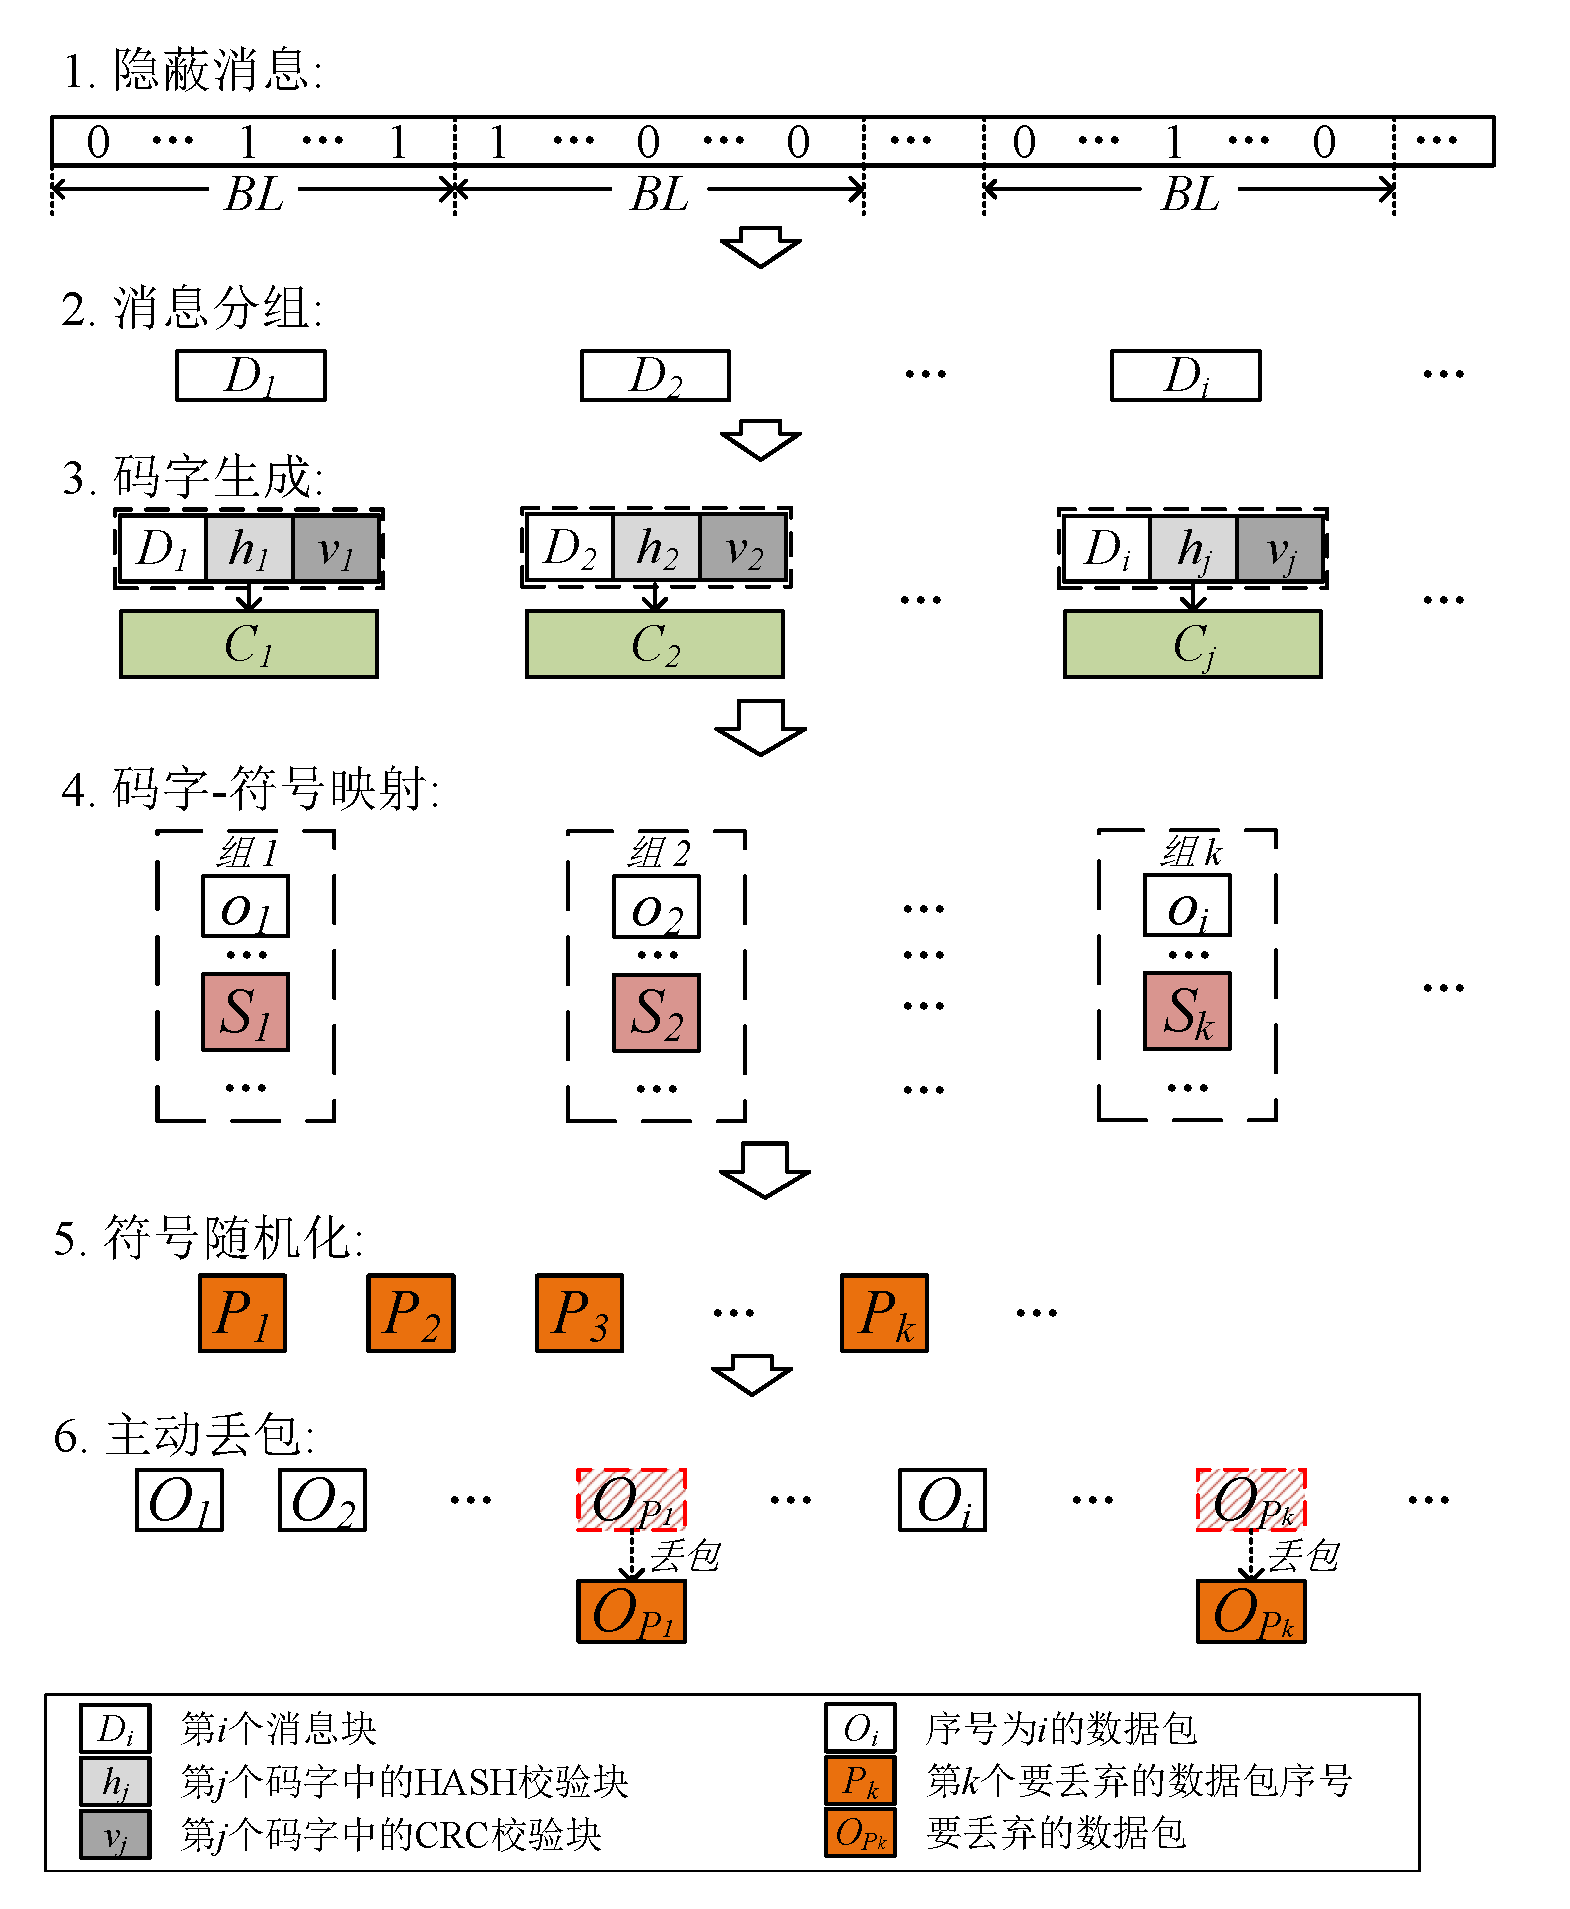
\includegraphics[width=0.85\textwidth]{chapters/chapter5/figures/modulation-flow.pdf}
        \caption{基于多重校验的时间隐通道调制流程}
        \label{fig:5:modulation-flow}
    \end{figure}

    \begin{figure}
        \centering
        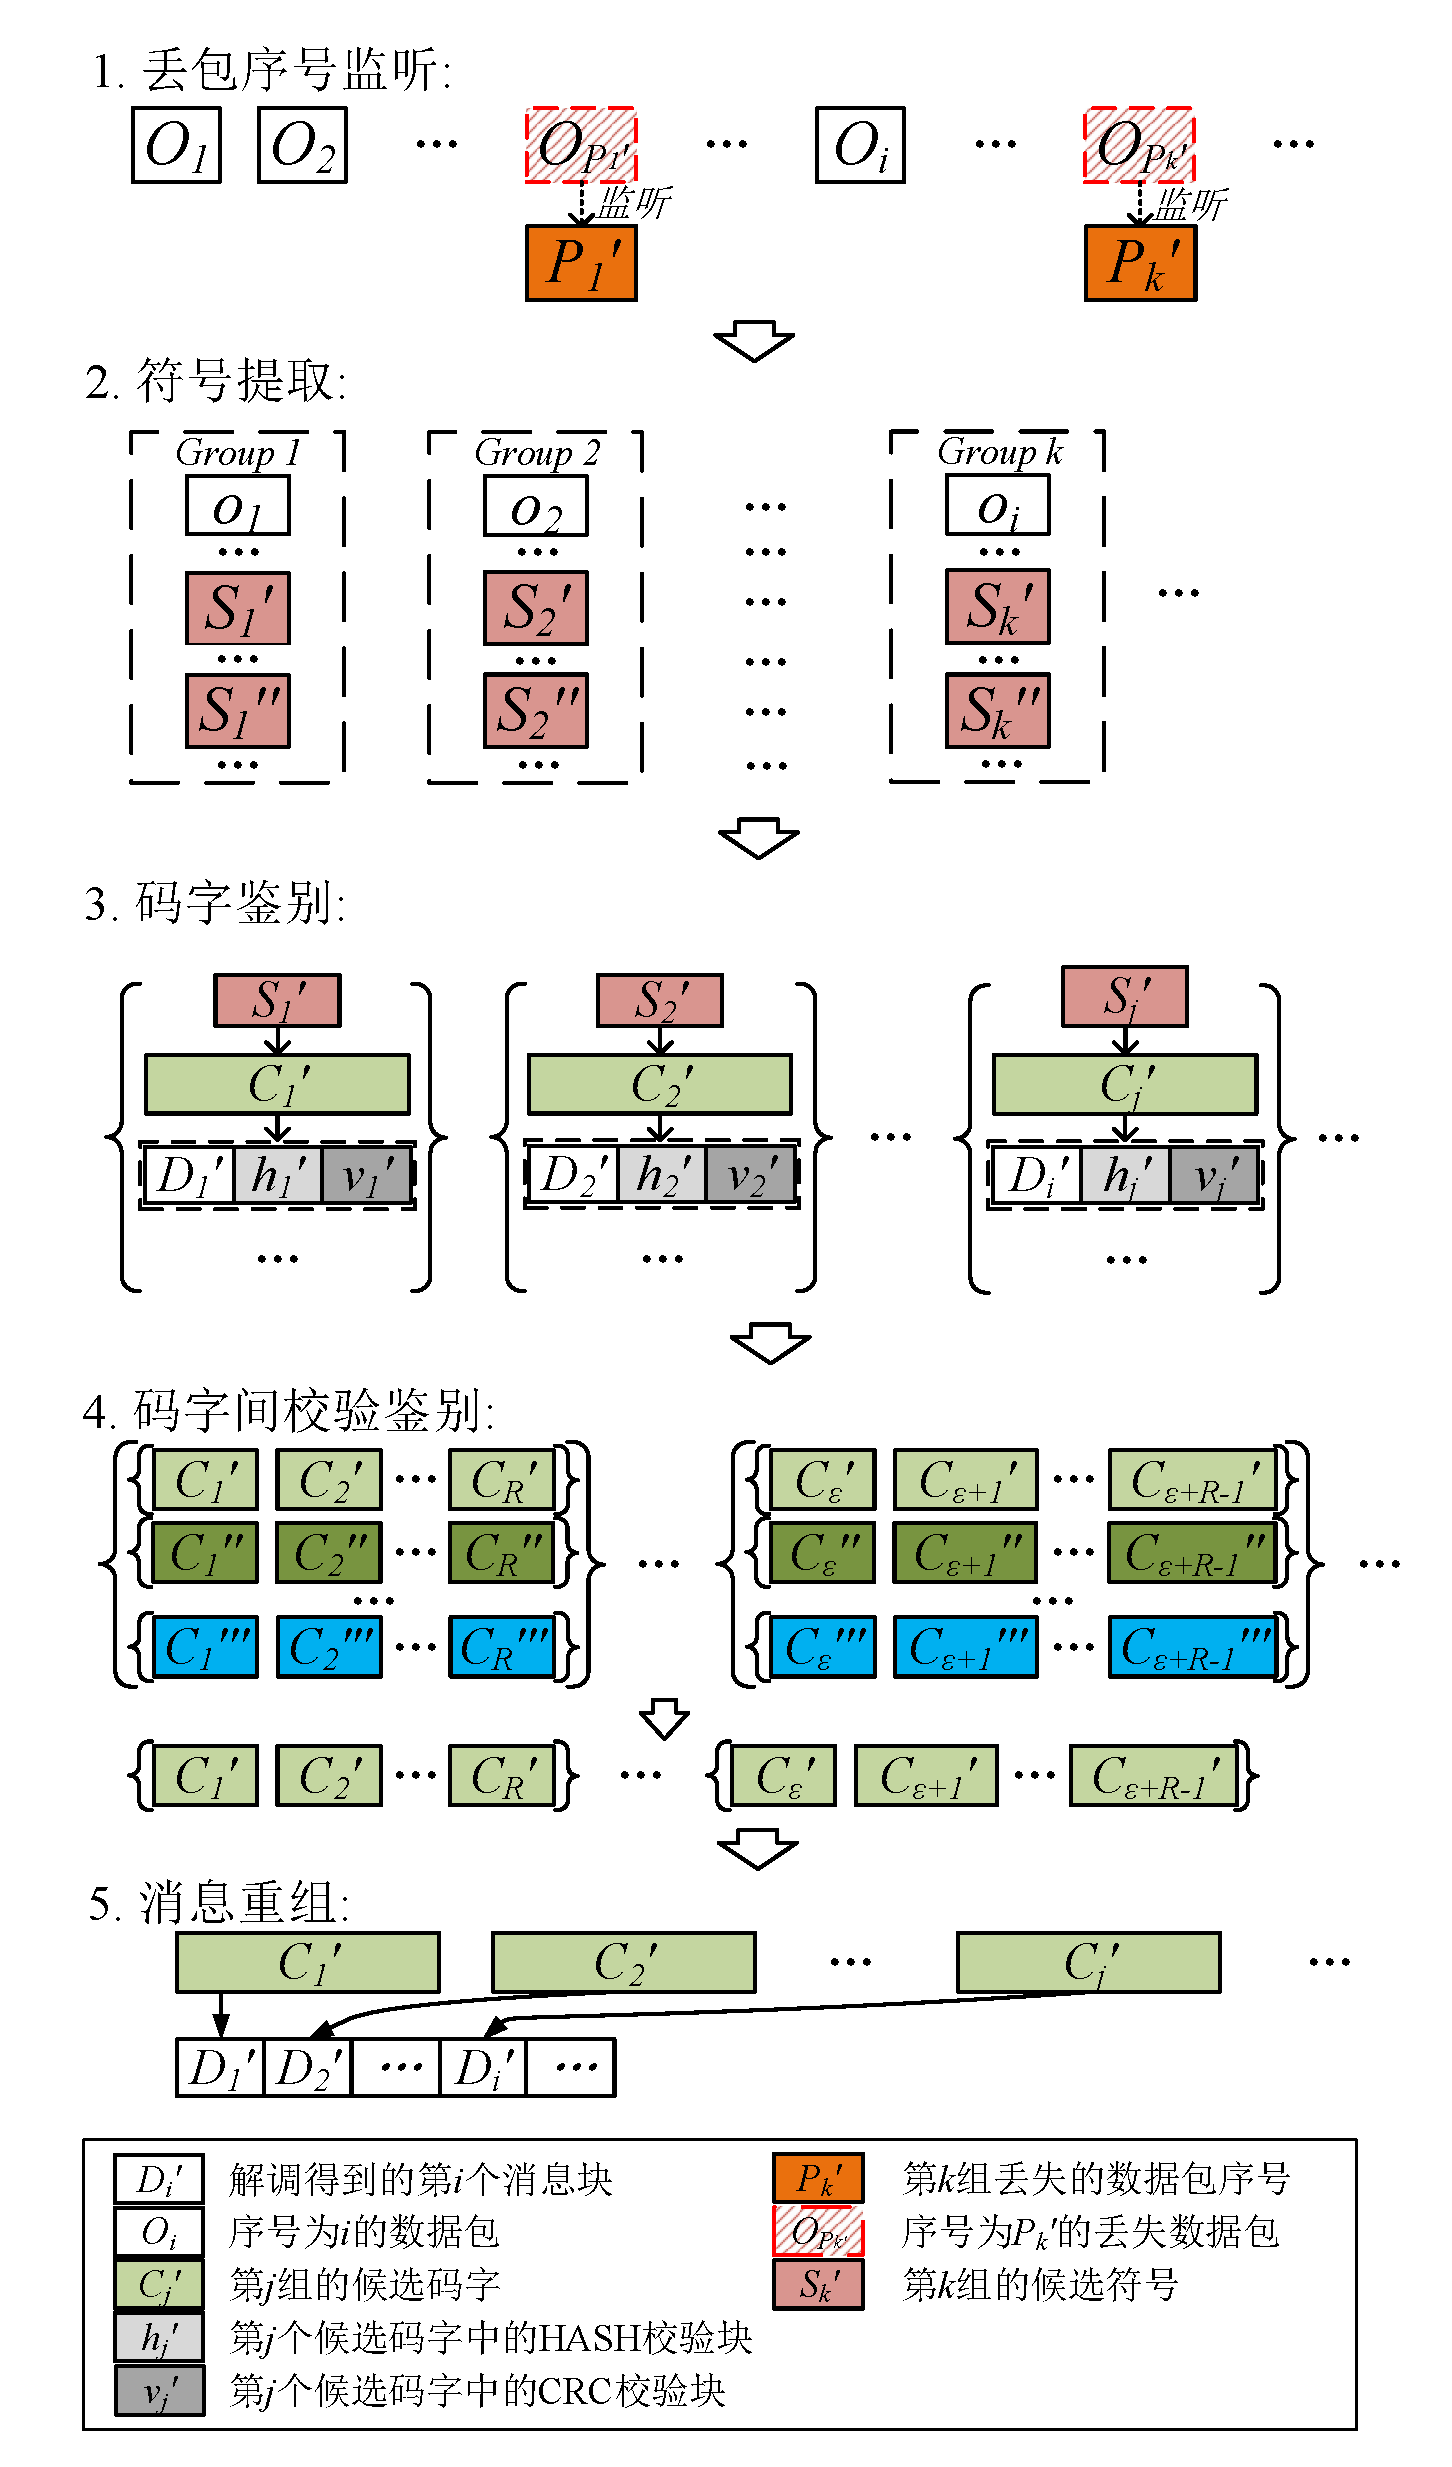
\includegraphics[width=0.75\textwidth]{chapters/chapter5/figures/demodulation-flow.pdf}
        \caption{基于多重校验的时间隐通道解调流程}
        \label{fig:5:demodulation-flow}
    \end{figure}
}

如图\nref{fig:5:modulation-flow},调制过程中的数据流变化主要分为5个部分,与时间隐通道架构中的调制流程基本一致。首先对隐蔽消息进行分组,每个数据块的长度为$BL$,得到等长数据块$\{D_{1},D_{2},\cdots , D_{i}\}$。接下来,在每个数据块的基础上,计算基于HASH的码字间校验,并将摘要结果中的$L_{HASH}$bit提取出来,作为$h_{j}$,拼接到$D_{i}$后部。对于每一个$\{D_{i}//h_{j}\}$组合,计算其CRC散列值,并将结果中的$L_{CRC}$bit作为$v_{j}$,将$\{D_{i},j_{j},v_{j}\}$按序组合,得到码字$C_{j}$。因此,$L_{Codeword}$与$BL$、$L_{HASH}$及$L_{CRC}$的关系,如公式(\nref{equ:5:codeword-length})。

\insertEquation{
    \begin{equation}
    \label{equ:5:codeword-length}
		L_{Codeword} = BL + L_{HASH} + L_{CRC}
    \end{equation}
}

码字符号映射操作,将二进制的码字$C_{j}$,转换为每组中的相对偏移量$S_{k}$。在映射矩阵中,添加额外的异或校验符号,因此最终$S_{k}$的数量要多于$C_{j}$的数量。接下来,进行符号随机化的过程,基于传入的随机数种子,迭代伪随机数发生器,为每一组符号添加随机偏移量。伪随机数发生器在保证种子一致的情况下,具有相同的随机数序列,因此保证随机数种子即可确保调制结果的随机性。通过结合用户自定义的随机数种子,及RTP中的SSRC随机字段,保证每次传输的丢包位置不同,抵御重放攻击、增强保密性。最后,将符号转换为数据包序号$P_{k}$,在主动丢包过程中,将具有序号$P_{k}$的数据包丢弃,调制过程结束。

调制过程中,影响时间隐通道抗检测能力的为参数$L_{Codeword}$,其取值决定了时间隐通道的丢包密度,通过增大$L_{Codeword}$从而获得更好的抗检测能力。影响鲁棒性的环节,包括码字生成中的参数$L_{HASH}$的$L_{CRC}$,设定更多的校验位数,即可降低码字的分布密度,噪声产生传输错误的概率降低。在保密性方面,主要由码字中的校验信息及符号中的随机偏移量两部分组成,生成$h_{j}$及$v_{j}$的源数据中均进行加盐操作,因此即使传输相同的隐蔽消息,每次生成的码字也完全不同;在随机偏移量部分,每个符号有其对应的偏移量,即使隐蔽消息不具备随机性,添加随机偏移量后具备随机特征。即使监听者获取了该时间隐通道的构建方案,并按照相同的方式进行破解,调制过程中产生的随机因素具有足够的安全保证。

\subsection{解调流程}
\label{chap:hash:results:demodulation}

如图\nref{fig:5:demodulation-flow},解调过程中的数据流程主要包括5个部分,与图\nref{fig:5:system-model}中解调过程对应。丢包序号监听分析当前接收到的数据包序号,根据序号之间的空缺情况,得到丢失数据包序号$P_{k}'$。符号提取过程将序号转变为每组的符号,在该时间隐通道中,网络噪声产生的干扰不可避免,每组中的候选符号存在不止一个的情况,因此每组的候选符号为集合$\{S_{k}',S_{k}'',\cdots \}$。

对于候选符号$\{S_{k}',S_{k}'',\cdots \}$,首先根据协商好的随机数种子,迭代伪随机数生成器,将每组符号中的随机偏移量消除,从而进行鉴别过程。在该方法的映射矩阵中,添加了对符号的异或校验,在提取符号的过程中,对异或校验关系进行验证,鉴别出符合规则的码字,进入码字鉴别过程。

码字鉴别过程,对码字中包含的$v_{j}$部分进行验证,判断符合规则的候选码字。接下来对码字中包含的$h_{j}$部分进行验证,按照码字间校验的模式,遍历所有的码字组合,出现校验失败则意味着组合无效。最终,得到一组具有最大概率的码字组合$\{C_{1}',C_{2}',\cdots, C_{j}'\}$,进入消息重组阶段。最后的消息重组过程,将码字中的数据块$D_{i}$提取出来,按照顺序组合得到隐蔽消息。

该时间隐通道构建方法,调制基础基于数据包序号,因此自身具有传输同步功能,无需同步时钟也可保证消息顺序。通过结合码字间校验、码字自校验、符号间校验及行优先映射矩阵,逐层降低噪声强度,提高时间隐通道的鲁棒性。
\section{鲁棒性方案设计}
\label{chap:hash:robustness}

\subsection{基于HASH的组间校验方案}
\label{chap:hash:robustness:hash}

\subsubsection{调制过程}
\label{chap:hash:robustness:hash:modulation}

\subsubsection{解调过程}
\label{chap:hash:robustness:hash:demodulation}

\subsection{基于CRC的码字自校验}
\label{chap:hash:robustness:crc}

\subsubsection{调制过程}
\label{chap:hash:robustness:crc:modulation}

\subsubsection{解调过程}
\label{chap:hash:robustness:crc:demodulation}

\subsection{基于异或的映射矩阵校验}
\label{chap:hash:robustness:xor}

\subsubsection{调制过程}
\label{chap:hash:robustness:xor:modulation}

\subsubsection{解调过程}
\label{chap:hash:robustness:xor:demodulation}

\section{实验结果及评估}
\label{chap:hash:result}

\subsection{实验环境及参数}
\label{chap:hash:result:parameters}

\subsection{抗检测能力测试}
\label{chap:hash:result:undetectability}

\subsubsection{IPD测试}
\label{chap:hash:result:undetectability:ipd}

\subsubsection{区间丢包率测试}
\label{chap:hash:result:undetectability:plr}

\subsubsection{突发丢包长度测试}
\label{chap:hash:result:undetectability:burst}

\subsection{鲁棒性测试}
\label{chap:hash:result:robustness}

\subsection{传输性能测试}
\label{chap:hash:result:throughput}

\subsection{构建代价}
\label{chap:hash:result:cost}

\subsection{综合评估}
\label{chap:hash:result:evaluation}

\subsection{结论}
\label{chap:hash:result:conclusion}
\section{本章小结}
\label{chap:hash:summary}

本章介绍了基于多重校验纠错的时间隐通道构建方法,重点降低隐通道的传输误码率。为提高时间隐通道鲁棒性,该方法采用了多重校验纠错模式,包括基于HASH的码字间校验、基于CRC的码字自校验以及基于异或的映射矩阵校验。经过实验测试表明,该时间隐通道在保证传输隐蔽性的前提下,通过灵活组织传输参数,能够在降低误码率的同时保证一定的传输性能。Excellent场景中,误码率低于{0.08\ \%}的情况下,同时保持{0.49\ bps}的传输性能,较本文\ \nref{chap:zigzag:model}中提出的方法有了提升。网络噪声较强的Good场景中,该方法虽然损失了一定的性能,但依然能够在误码率低于{1\ \%}的情况下保持{0.2\ bps}的传输性能,有效证明了多重校验纠错的有效性。

在保密性方面,通过结合用户共享信息及RTP头中的随机字段,实现散列值计算过程的加盐。同时,通过迭代伪随机数生成器,对每一组符号添加随机偏移量。从而保证即使相同的数据,在不同时刻产生的丢包位置也不完全相同。另一方面,即使监听者知晓了传输原理,由于缺乏传输参数等关键信息,反向破解复杂度较高,隐蔽消息得到保护。对于主动式监听者来说,只有将与序号相关的所有字段进行重设,才能完全阻止该时间隐通道。

因此,基于多重校验纠错的时间隐通道构建方法,在抗检测能力、鲁棒性、保密性、调制代价及传输性能各方面,均满足了时间隐通道指标的要求。